\section{accessibilita}
Le immagini nel nostro sito risultano essere prevalentemente immagini di contenuto poiche' mostrano effettivamente all'utente come si presenta il nostro centro sportivo all'interno o come si presentano i nostri campi da gioco che andra' a prenotare, abbiamo scelto di assegnare ai tag \textbf{alt} delle immagini frasi del tipo:"il capo da calcetto" poiche' descriverlo risulta impossibile.
Abbiamo fatto diversi test in internet per testare il nostro sito per le persone che soffrono di daltonismo, qui sotto possiamo vedere qualche immagine filtrata tramite su \textbf{http://colorfilter.wickline.org/} per fare i test \newline
\begin{figure}
	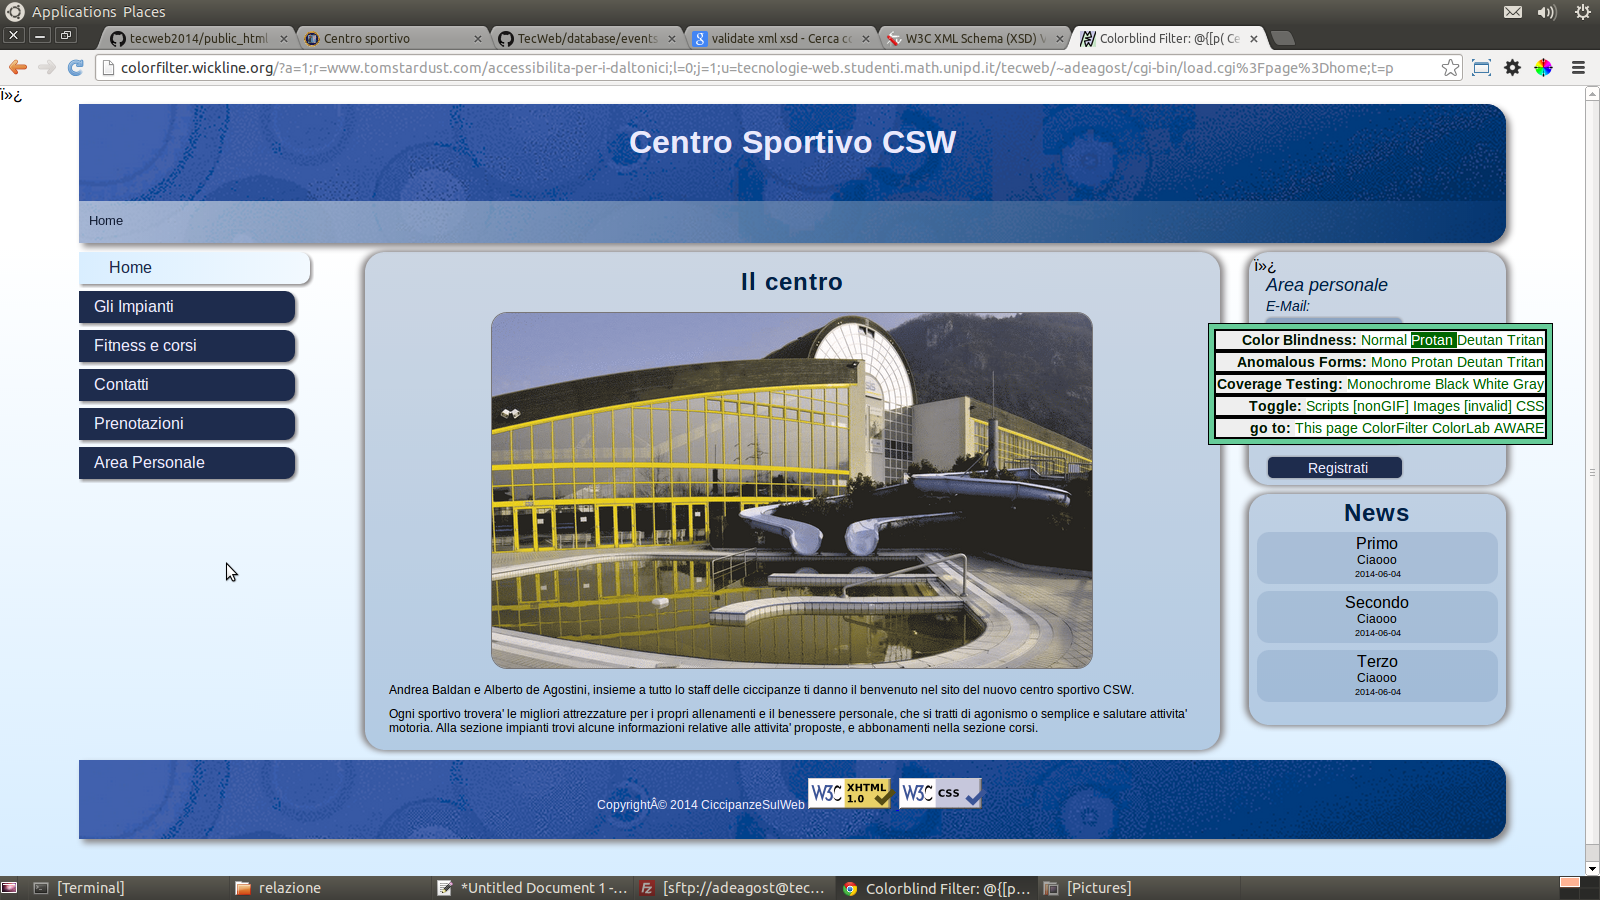
\includegraphics[height=0.5\textwidth]{images/protan.png} 
	\caption{a) protanopia}
\end{figure}
\begin{figure}
	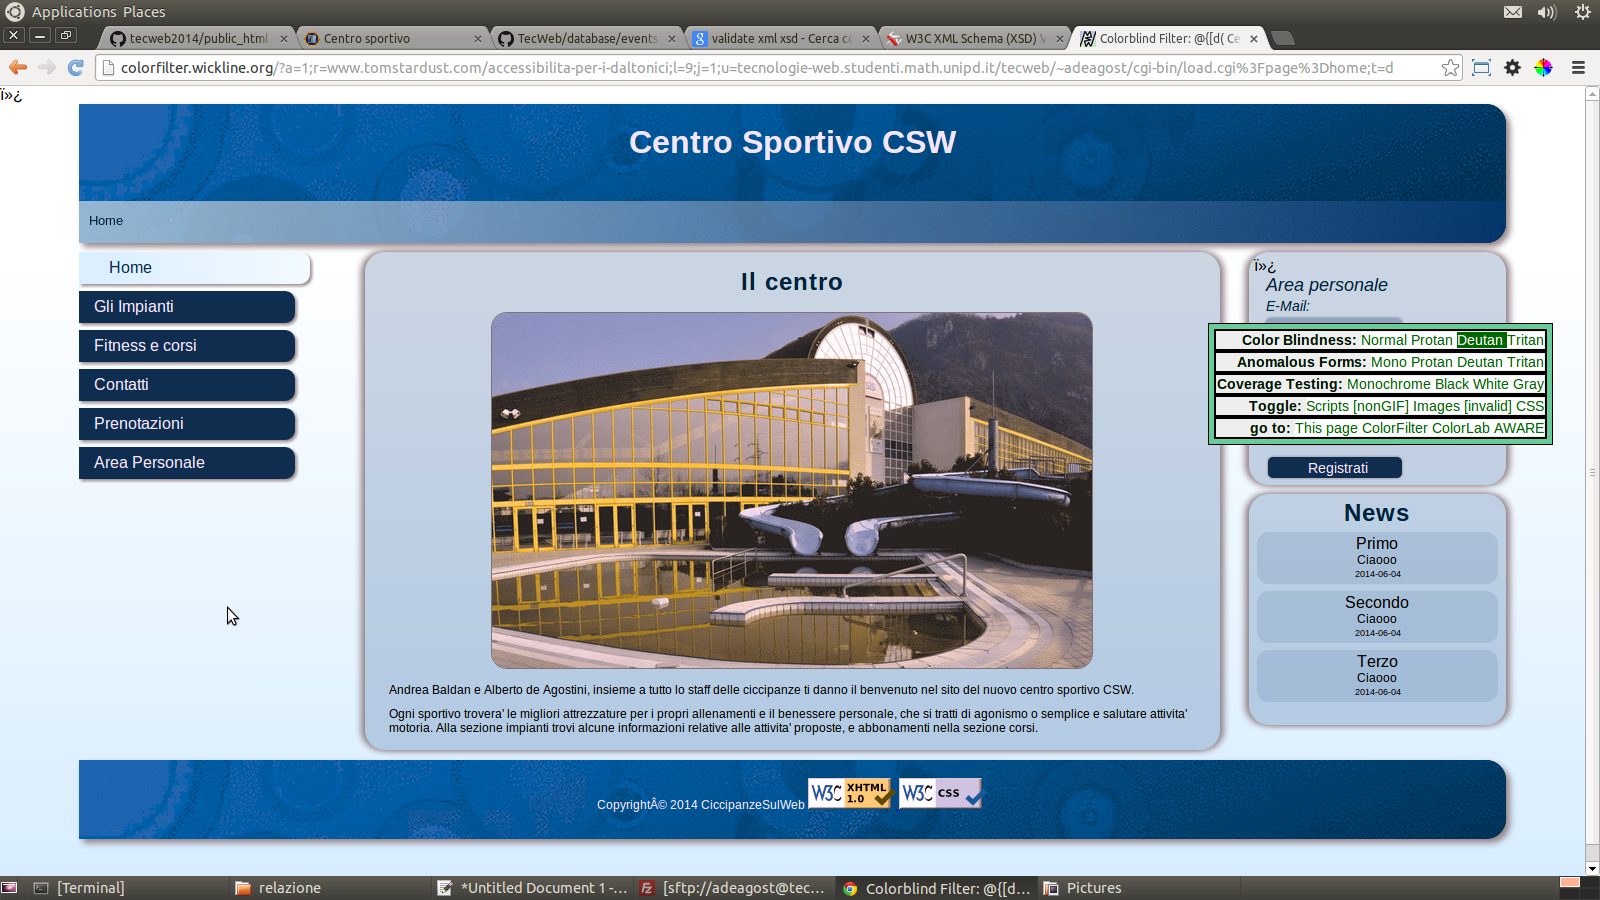
\includegraphics[height=0.5\textwidth]{images/deutran.png} 
	\caption{b) deutranopia} 
\end{figure}
\begin{figure}
	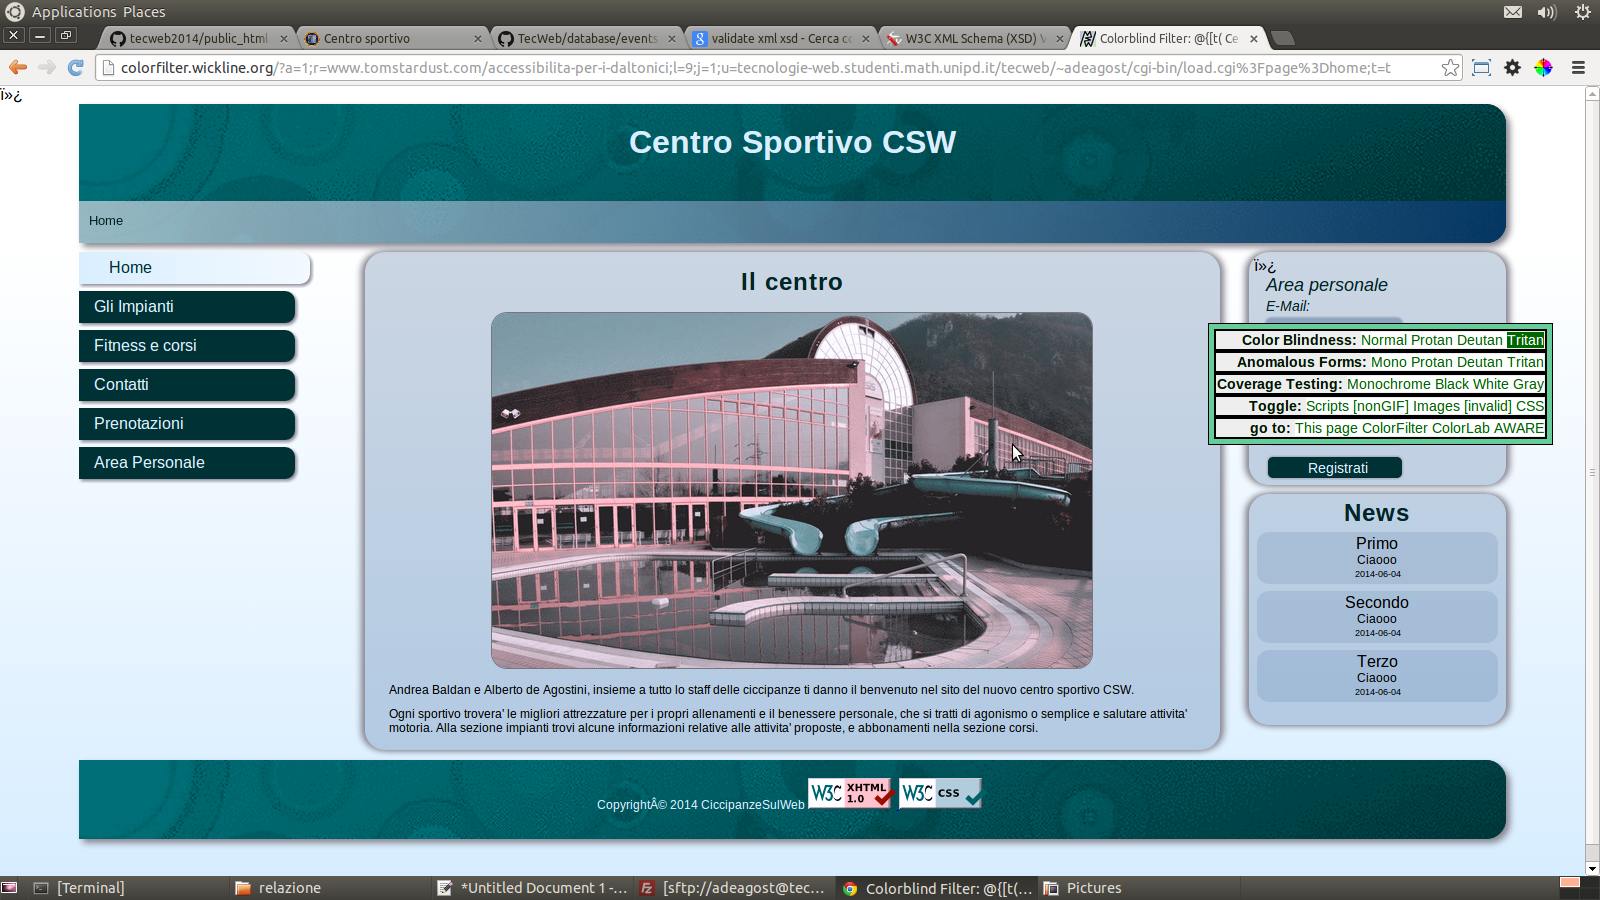
\includegraphics[height=0.5\textwidth]{images/tritan.png} 
	\caption{c) tritanopia}
\end{figure}
abbiamo allegato solo poche immagini visto che i colori utilizzati nel sito sono sempre gli stessi.\newline
Abbiamo controllato anche il contrasto del sito su \textbf{http://gmazzocato.altervista.org/colorwheel/wheel.php} per scegliere colori con contrasto ratio sempre maggiore di 7 per avere un punteggio di AAA. Su quel sito si puo' vedere anche il contrasto sempre per le persone che soffrono di protanopia, deutranopia e tritanopia.
